%%%%%%%%%%%%%%%%%%%%%%%%%%%%%%%%%%%%%%%%%
% The Legrand Orange Book
% LaTeX Template
% Version 2.1.1 (14/2/16)
%
% This template has been downloaded from:
% http://www.LaTeXTemplates.com
%
% Original author:
% Mathias Legrand (legrand.mathias@gmail.com) with modifications by:
% Vel (vel@latextemplates.com)
%
% License:
% CC BY-NC-SA 3.0 (http://creativecommons.org/licenses/by-nc-sa/3.0/)
%
% Compiling this template:
% This template uses biber for its bibliography and makeindex for its index.
% When you first open the template, compile it from the command line with the 
% commands below to make sure your LaTeX distribution is configured correctly:
%
% 1) pdflatex main
% 2) makeindex main.idx -s StyleInd.ist
% 3) biber main
% 4) pdflatex main x 2
%
% After this, when you wish to update the bibliography/index use the appropriate
% command above and make sure to compile with pdflatex several times 
% afterwards to propagate your changes to the document.
%
% This template also uses a number of packages which may need to be
% updated to the newest versions for the template to compile. It is strongly
% recommended you update your LaTeX distribution if you have any
% compilation errors.
%
% Important note:
% Chapter heading images should have a 2:1 width:height ratio,
% e.g. 920px width and 460px height.
%
%%%%%%%%%%%%%%%%%%%%%%%%%%%%%%%%%%%%%%%%%

%----------------------------------------------------------------------------------------
%	PACKAGES AND OTHER DOCUMENT CONFIGURATIONS
%----------------------------------------------------------------------------------------

\documentclass[11pt,fleqn]{book} % Default font size and left-justified equations

%\usepackage{amsmath,amssymb}
%\usepackage{mathpazo}
%\usepackage[utf8]{inputenc}
%\usepackage[spanish]{babel}
%\usepackage{graphicx}
%\usepackage{gb4e}

%----------------------------------------------------------------------------------------


\usepackage{multicol}
\usepackage{array,booktabs,tabularx}
\usepackage{graphicx}
\usepackage{tikz}
\usetikzlibrary{arrows,shapes,trees,automata}
\usepackage{pgfplots}
\usepackage{float}
\usepackage{float}
\usepackage{subfigure}
\usepackage{xcolor}
\usepackage{pifont}
\usepackage{makeidx}
\makeindex
\usepackage{tocbibind}
\usepackage{hyperref}
\usepackage{pdfpages}


%---------------------------------------------------------------------------------------
\title{ Ecuaciones Diferenciales Ordinarias.}
\author{Pedro Miramontes\\ Augusto Cabrera Becerril\\ Ulises Rayón}
\date{\today}

%-----------------------------------------------------------------------------------------
\newtheorem{definicion}{Definición}
\newtheorem{ejemplo}{Ejemplo}
\newtheorem{teorema}{Teorema}
\newtheorem{lema}{Lema}
\newtheorem{prop}{Proposición}
\newtheorem{af}{Afirmación}
\newtheorem{coro}{Corolario}
\newtheorem{obs}{Observación}
\newtheorem{casos}{Caso}
 \renewcommand{\spanishrefname}{Bibliografía.}
\renewcommand{\spanishproofname}{Prueba.}
\decimalpoint
\pagestyle{fancy}
\def\sectionautorefname{section}
 % Insert the commands.tex file which contains the majority of the structure behind the template

\begin{document}

%----------------------------------------------------------------------------------------
%	TITLE PAGE
%----------------------------------------------------------------------------------------
\maketitle
%\begingroup
%\thispagestyle{empty}
%\begin{tikzpicture}[remember picture,overlay]
%\coordinate [below=12cm] (midpoint) at (current page.north);
%\node at (current page.north west)
%{\begin{tikzpicture}[remember picture,overlay]
%\node[anchor=north west,inner sep=0pt] at (0,0) {
%
\includegraphics[width=\paperwidth]{background}
%}; % Background image
%\draw[anchor=north] (midpoint) node %[fill=ocre!30!white,fill opacity=0.6,text %opacity=1,inner %sep=1cm]{\Huge\centering\bfseries\sffamily\parbox[c][][t]{\paperwidth}{\centering Ecuaciones Diferenciales\\[15pt] % Book title
%{\Large Una introducci\'on a la dinámica no lineal}\\[20pt] % Subtitle
%{\huge Pedro Miramontes\\ Augusto Cabrera Becerril\\ Ulises Rayón}}}; % Author name
%\end{tikzpicture}};
%\end{tikzpicture}
%\vfill
%\endgroup

%----------------------------------------------------------------------------------------
%	COPYRIGHT PAGE
%----------------------------------------------------------------------------------------

%\newpage
%~\vfill
%\thispagestyle{empty}

%\noindent %Copyright \copyleft\ 2019 John Smith\\ % Copyright notice

%\noindent \textsc{Published by Publisher}\\ % Publisher

%\noindent \textsc{book-website.com}\\ % URL

%\noindent Licensed under the Creative Commons Attribution-NonCommercial 3.0 Unported License (the ``License''). You may not use this file except in compliance with the License. You may obtain a copy of the License at \url{http://creativecommons.org/licenses/by-nc/3.0}. Unless required by applicable law or agreed to in writing, software distributed under the License is distributed on an \textsc{``as is'' basis, without warranties or conditions of any kind}, either express or implied. See the License for the specific language governing permissions and limitations under the License.\\ % License information

%\noindent \textit{First printing, March 2013} % Printing/edition date

%----------------------------------------------------------------------------------------
%	TABLE OF CONTENTS
%----------------------------------------------------------------------------------------

%\usechapterimagefalse % If you don't want to include a chapter image, use this to toggle images off - it can be enabled later with \usechapterimagetrue

%\chapterimage{chapter_head_1.pdf} % Table of contents heading image

%\pagestyle{empty} % No headers

\tableofcontents % Print the table of contents itself

%\cleardoublepage % Forces the first chapter to start on an odd page so it's on the right

%\pagestyle{fancy} % Print headers again

%----------------------------------------------------------------------------------------
%	PART
%----------------------------------------------------------------------------------------

\part{Primera Parte}

%----------------------------------------------------------------------------------------
%	Capitulo 1
%----------------------------------------------------------------------------------------

%\chapterimage{chapter_head_2.pdf} % Chapter heading image

\chapter{Una nota histórica}

%----------------------------------------------------------------------------------------
%	Capitulo 2
%----------------------------------------------------------------------------------------

\chapter{Ecuaciones Diferenciales de Primer Orden:
        Lineales y no Lineales}

\section{Una idea intuitiva}\index{Una idea intuitiva}

Supongamos que tenemos los siguientes datos de una población de bacterias:
%%Datos
La gráfica de los datos luce de la siguiente manera:
%%Gráfica
Ahora, notemos que podemos calcular, dado los datos, la pendiente entre cualesquiera
dos puntos. La pendiente es:
\begin{equation}
    m_{i} = \displaystyle\frac{\Delta y_{i}}{\Delta t_{i}} = \frac{y_{i+1}-y_{i}}{t_{i+1}-t_{i}}
\end{equation}


Ahora, de alguna forma lo que esto nos quiere decir es que existe una curva $x(t)$ que evaluada en el intervalo $\delta t_{i}$ tiene una pendiente $x'(\Delta t_{i}) = m_{i} $. 
\ \\
\noindent
En realidad hay muchas curvas que cumplen que $x'(\Delta t_{i}) = m_{i}$ sin embargo existe sólo una curva que además de eso $x(t_{i}) = p_{i}$. Notemos que además esta relación define una relación biyectiva entre los datos del tiempo y el tamaño de la población, podemos aventurarnos a decir que el dominio de la curva $x(t)$ es justamente los el conjunto $T = \left\{ t : t \in [0,15]\subset \mathbb{R}\right\}$ y la imagen son todos los puntos correspondientes a la población. 
\ '\\
\noindent
Ahora bien, consideremos los datos que se reportan de otro experimento
\section{Procesos a tasa constante}

En la Naturaleza existe una gran cantidad de procesos que a lo largo del tiempo cambian o evolucionan a {\it tasa constante}. En esta sección haremos las definiciones esenciales y en las próximas veremos ejemplos de ellos.

Sin embargo, primero queremos precisar que cuando hablemos de {\it Naturaleza } entenderemos que comprende al mundo vivo --humano o no humano-- y los fenómenos que involucran a la materia inerte.

Vamos a  comenzar por lo básico. Supongamos que tenemos una magnitud $p(t)$ que es función del tiempo. Dicha magnitud puede representar a cualquier variable de interés de estudio: tamaño de una población, cantidad de dinero, número de enfermos, cantidad de material radioactivo, etcétera. Empezaremos por suponer que $p(t)$ solamente puede evaluarse en valores discretos del tiempo por lo cual es de interés estudiar la sucesión:
\[
\{p(t)\}_{t=0}^n = p(0),p(1),p(2),\hdots p(n)
\]
\noindent donde $n$ es un valor arbitrario del tiempo.


\[
 \dfrac {p(n+1) -p(n) }{p(n)}=q\\
 \]


\section{Modelos simples de poblaciones}

Consideremos la hipótesis siguiente: Cierta población de seres vivos crece de forma proporcional al tamaño de la población actual. Si llamamos $X(t)$ al tamaño de la población actual entonces un mecanismo de crecimiento como el que se propone esta descrito por la siguiente ecuación:

\begin{equation}
    \frac{\mathrm{d}X}{\mathrm{d}t}=\rho X(t)
\end{equation}
donde $\rho\neq 0$ es la tasa de nacimientos per cápita

La ecuación anterior es equivalente a la ecuación integral:

\begin{equation}
    \int_{X(0)}^{X(t)} \frac{\mathrm{d}X}{X} = \rho\int_0^t \mathrm{d}\tau 
\end{equation}

Si llamamos $X_0=X(0)$ a la población inicial, tenemos por el teorema fundamental del Cálculo:

\begin{equation}
    \ln (X(t))-\ln(X_0)=\rho(t)
\end{equation}

o bien:

\begin{equation}
    \ln (X(t))=\ln(X_0)+\rho(t)
\end{equation}

Tomando exponencial de ambos lados, obtenemos:
\begin{equation}
  X(t)= X_0 e^{\rho t} 
\end{equation}

Es decir que si la población cambia de forma proporcional a su tamaño actual, entonces esta crece de forma exponencial. El comportamiento predicho por este modelo es poco razonable. 

El inglés Malthus propuso este modelo en el siglo XIX. Su argumento era que mientras los recursos (la comida, etc) se producida con una tasa geométrica, el crecimiento de la población es exponencial y por tanto crece indefinidamente. 



\section{La separación de variables}

Para la ecuación del crecimiento malthusiano utilizamos que la ecuación $\dfrac{\mathrm{d}X}{\mathrm{d}t}=\rho X$ es equivalente a 
$$\int \dfrac{\mathrm{d}X}{X}=\int \rho\mathrm{d}t$$
Esta idea es una técnica estándar para resolver cierta clase de ecuaciones, llamadas de variables separadas, veamos algunos ejemplos antes de dilucidar por qué funciona el truco de la separación de variables.

\begin{exampleT}
Consideremos la ecuación $\dfrac{\mathrm{d}Y}{\mathrm{d}X}=-\dfrac{X}{Y}$ esta ecuación diferencial es equivalente a la ecuación integral 
$$
\int Y\mathrm{d}Y =-\int X\mathrm{d}X
$$
integrando formalmente tenemos
$$
Y^2+X^2=\xi
$$
para alguna constante no-negativa $\xi$, las soluciones de este problema son círculos de radio $\xi$ .
\begin{figure}[H]
    \centering
    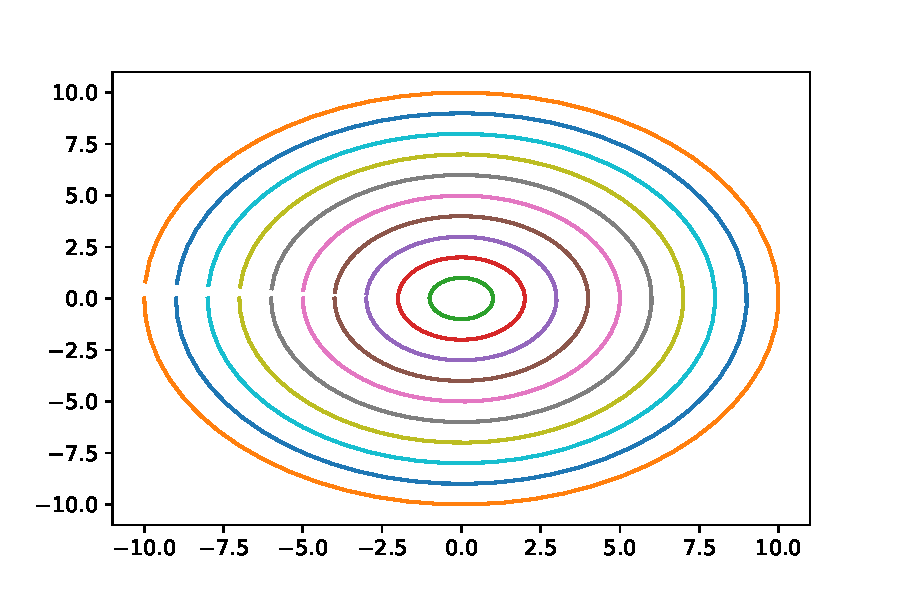
\includegraphics[scale=0.85]{circulos.pdf}
    \caption{Soluciones para el problema $\dfrac{\mathrm{d}Y}{\mathrm{d}X}=-\dfrac{X}{Y}$ }
    \label{fig:circ}
\end{figure}
\end{exampleT}

\begin{exampleT}
Consideremos la ecuación $\dfrac{\mathrm{d}Y}{\mathrm{d}X}=\dfrac{Y}{X}$ esta ecuación diferencial es equivalente a la ecuación integral 
$$
\int \dfrac{\mathrm{d}Y}{Y} =-\int \dfrac{\mathrm{d}X}{X}X
$$
integrando formalmente tenemos
$$
\ln(Y)=\ln(X)+\xi
$$
es decir
$$
Y(X)=e^{\xi}X
$$
\begin{figure}[H]
    \centering
    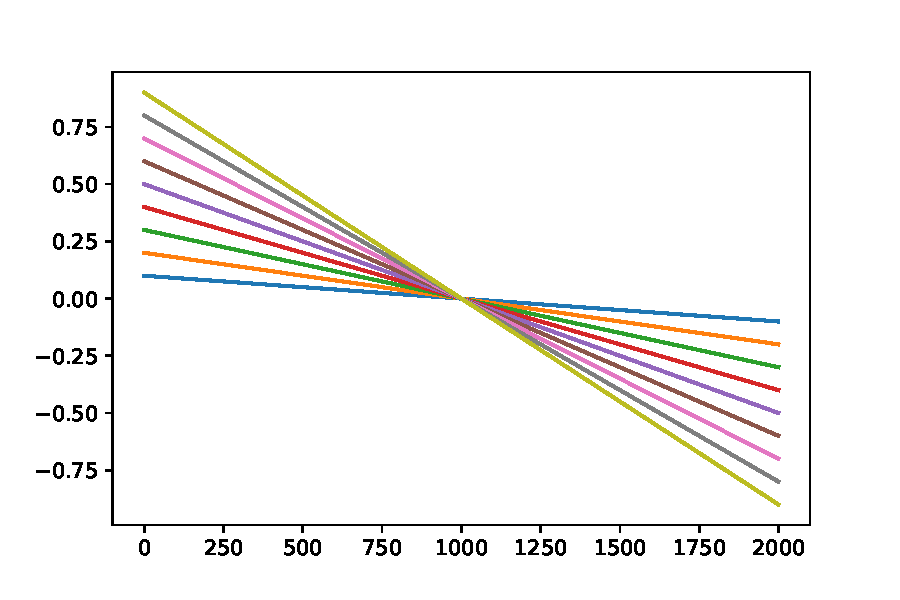
\includegraphics[scale=0.85]{ejemplo2.pdf}
    \caption{Soluciones para el problema $\dfrac{\mathrm{d}Y}{\mathrm{d}X}=\dfrac{Y}{X}$ para distintas condiciones iniciales}
    \label{fig:ej2}
\end{figure}
\end{exampleT}
 
 Las ecuaciones que están dadas en la forma $\dfrac{\mathrm{d}Y}{\mathrm{d}X}=\dfrac{\Psi(X)}{\Phi(Y)}$ son llamadas de variables separadas, suponiendo que $\Psi$y $\Phi$ son continuas en el dominio correspondiente, entonces la ecuación integral
 $$
 \int\Phi(Y)\mathrm{d}Y=\int\Psi(X)\mathrm{d}X+\xi
 $$
 Esta ecuación integral es llamada finita (¿Se imagina por qué?) y también la satisfacen las soluciones de la ecuación diferencial. Una función de la forma $\Omega(x,y)=0$ que determina a $Y(X)$ como función implícita es llamada integral de la ecuación diferencial, si además esta función determina sin excepción  a todas las soluciones de la ecuación se llama una integral general.
 
 Si $Y(X_0)=Y_0$ es una condición inicial, entonces la integral
 $$
 \int_{Y_0}^{Y}\Phi(Y)\mathrm{d}Y=\int_{X_0}^{X}\Psi(X)\mathrm{d}X
 $$
determina de manera unívoca la solución.

\begin{figure}[H]
    \centering
    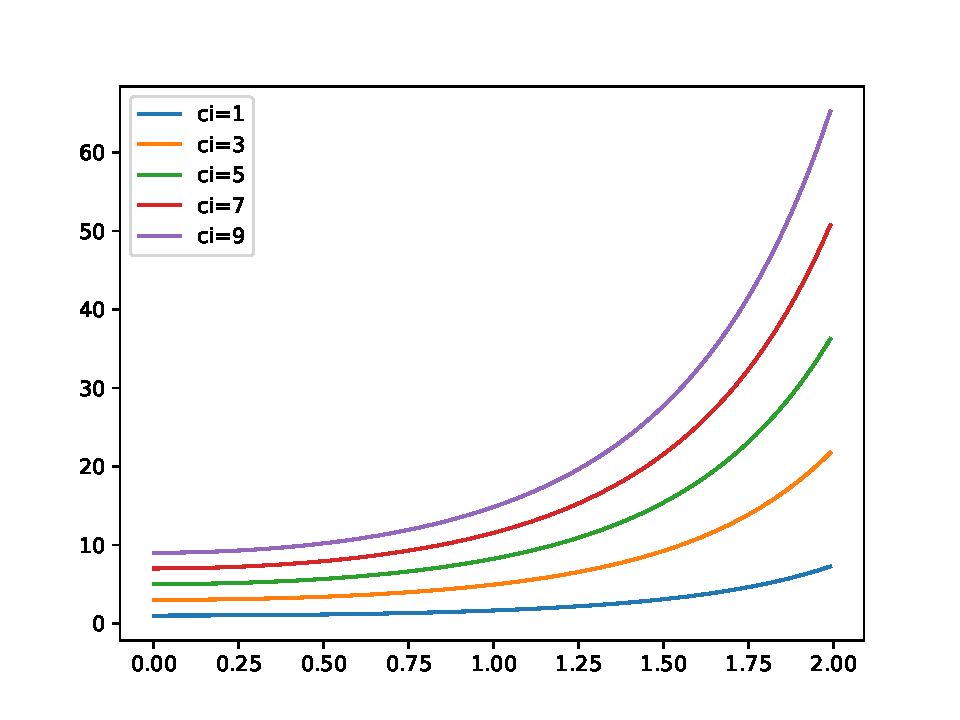
\includegraphics[scale=0.85]{exponenciales1.pdf}
    \caption{Soluciones de la ecuación de Malthus para distintos valores iniciales}
    \label{fig:exposci}
\end{figure}

Dada una condición inicial, para el problema del crecimiento exponencial, hay una solución única, para un valor fijo del parámetro $\rho$, ahora variaremos un poco este parámetro. Tenemos el siguiente comportamiento. 
\begin{enumerate}
    \item Para $\rho=0$ la solución es constante, en general una solución constante es llamada estacionaria.
    \item Para $\rho > 0$ El modelo describe u8n crecimiento ilimitado.
    \item Para $\rho<0$ El modelo describe un decrecimiento asintótico a cero. Podemos representar el cambio cualitativo de las soluciones cuando variamos  el parámetro mediante la llamada linea fase.
\end{enumerate}

\begin{figure}[H]
    \centering
    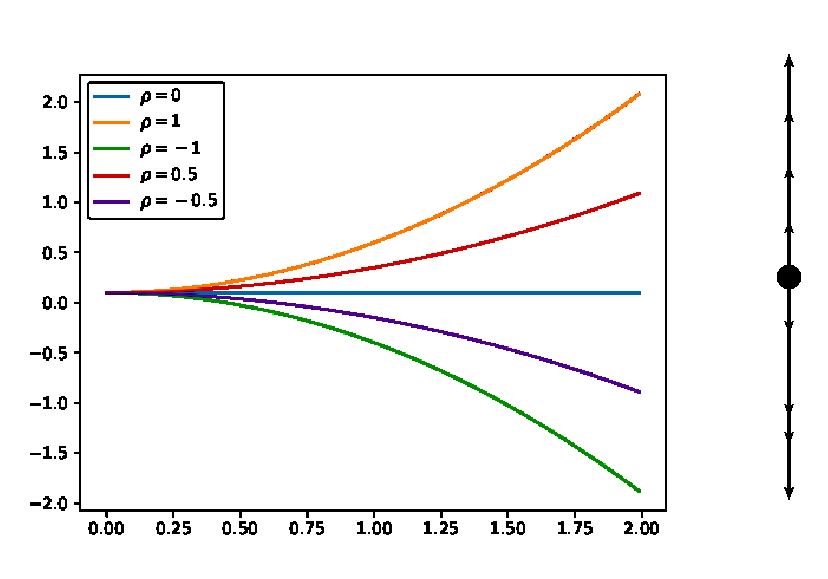
\includegraphics[scale=0.85]{exponenxiales2.pdf}
    \caption{distintos valores para el parámetro $\rho$}
    \label{fig:exposrho}
\end{figure}


Ahora pensemos en la siguiente ecuación>
$$
\varphi_1(x)\psi(y)\mathrm{d}x=\varphi_2(x)\psi_2(y)\mathrm{d}y
$$
no es una de variables separadas. Ahora si tenemos garantizado que : $\varphi_2(x)\neq 0$ y $\psi_2(y)\neq 0$, podemos  considerar la ecuación equivalente
$$
\frac{\varphi_1(x)}{\varphi_2(x)}\mathrm{d}x=\frac{\psi_1(y)}{\psi_2(y)}\mathrm{d}y
$$
que si es de variables separadas. A este tipo de ecuación se le llamda de variables separables.

Ahora hagamos un par de ejemplos sencillos:

\begin{exampleT}
Consideremos la ecuación

$$
x(1+y^2)\mathrm{d}x-y(1+x^2)\mathrm{d}y=0
$$
está garantizado que  tanto $1+y^2$ como $1+x^2$ son estríctamente positivos, así que nuestra ecuación es equivalente a la ecuación de variables separadas
$$
\frac{y}{1+y^2}\mathrm{d}y=\frac{x}{1+x^2}\mathrm{d}x
$$
que a su vez es equivalente a la ecuación integral
$$
\int \frac{y}{1+y^2}\mathrm{d}y=\int \frac{x}{1+x^2}\mathrm{d}x
$$
cuya solución es 
$$
\ln(1+y^2)-\ln(1+x^2)=\xi
$$
y finalmente, tomando exponencial en ambos términos de la ecuación
$$
\frac{1+y^2}{1+x^2}=e^{\xi}=\zeta
$$
\end{exampleT}

\begin{exampleT}
La ecuación
$$
\dot{x}=4t\sqrt{x}
$$
con condición inicial $x(1)=1$ es de variables separables puesto que $\sqrt(x)$ no se anula si empezamos en $1$. Nuestra ecuación es equivalente a:
$$
\frac{\mathrm{d}x}{2\sqrt{x}}=2t\mathrm{d}t
$$
asi que
$$
\int_{1}^{x}\frac{\mathrm{d}\xi}{2\sqrt{\xi}}=\int_{1}^{t}2\tau\mathrm{d}\tau
$$
y finalmente
$$
x(t)=t^4
$$
\end{exampleT}
\section{Decaimiento radioactivo}

La velocidad  de la desintegración radioactiva es proporcional a la cantidad $x$ de sustancia no desintegrada. Supongamos que en un momento inicial $t_0$ tenemos una masa $x(t_0)$ y $k$ es el coeficiente de desintegración, el fenómeno queda descrito por el siguiente problema de valores iniciales

\begin{eqnarray}
\dot{x}&=&-kx\\
x(t_0)&=&x_0
\end{eqnarray}

La solución para este problema de valores iniciales ya la conocemos
$$
x(t)=x_0e^{-k(t-t_0)}
$$

Ahora qué tanta información obtenemos del conocimiento de esta solución. Podemos calcular el tiempo en el cual ya se ha desintegrado la mitad de la masa inicial. Haciendo $\tau=t-t_0$ tenemos:
$$
\frac{x_0}{2}=x_0e^{-k\tau}
$$
 así, tomando $x_0 =1$
 $$
 \frac{1}{2}=e^{-k\tau}
 $$
  y finalmente
  $$
  \ln(\frac{1}{2})=-k\tau
  $$
  o equivalentemente
  $$
  \tau=\frac{\ln 2}{k}
  $$
  
  
\section{Problemas de mezclado}
\section{Un modelo de poblaciones más realista}

En la primera sección vimos que el modelo propuesto por Malthus  además de ser políticamente malintencionado, es a todas luces equivocado, ninguna población puede crecer permanente e ilimitadamente. Cualquier población ve acotado su crecimiento por cierta ``presión'' ejercida por el ambiente. ¿Cómo modelamos esta ``presión''? El problema es ahora proponer un modelo para una población cuyo crecimiento quede acotado por su propia dinámica. Llamemos $K$ a tal presión ambiental, en la literatura se le llama capacidad de carga del sistema, representa la cantidad de individuos de cierta población, a los que el medio puede proveer de subsistencia. Nuevamente consideraremos que la tasa intrínseca (natural) de crecimiento de la población es $\rho$ y que el crecimiento es proporcional no sólo al tamaño de la población actual, sino que decrece proporcionalmente a la proporción entre la población actual y la capacidad de carga.

\begin{equation}
    \dot{x}=\rho(1-\frac{x}{K})x
\end{equation}

Lo primero que debemos notar es que esta ecuación ya no es lineal en $x$, tiene un término cuadrático que de alguna forma nos da información sobre las interacciones intraespecíficas de la población. Ahora busquemos las soluciones de equilibrio, es decir aquellas para las cuales no hay cambios en la población. En este caso es claro que cuando $x=0$ ó $\left(1-\dfrac{x}{K}\right)=0$, entonces $\dot{x}\equiv 0$. Al caso  $x=0$ lo llamaremos el equilibrio trivial, y corresponde a que no hay ningún cambio en la población, cuando   $\left(1-\dfrac{x}{K}\right)=0$ tenemos que $x\equiv K$, es decir que al alcanzar la capacidad de carga del sistema el crecimiento se detiene. 

Consideremos la función polinomial $x\mapsto \rho(1-\frac{x}{K})x$ es una cuadrática cóncava en la dirección negativa del eje $\mathrm{Y}$, que cruza al eje horizontal en los puntos $(0,0)$ y $(0,K)$ el punto máximo de la parábola $\rho x-\rho \dfrac{x^2}{K}=0$ se alcanza cuando $\rho-2\rho \dfrac{x}{K}=0$ o equivalentemente $x=\dfrac{K}{2}$, así para distintos valores de $K$, el máximo de la parábola está más o menos alejado de la gráfica de la identidad. Las soluciones de la ecuación se alejan del $(0,0)$ y se aproximan a $(0,K)$. 

Nótese que si la condición inicial es menor que el parametro $K$, entonces . Ahora si iniciamos en una condición $x_0 > K$ entonces el cociente $\dfrac{x_0}{K}>1$ y la derivada $\dot{x} < 0$ y por lo tanto las soluciones son decrecientes y en ambos casos se aproximan asintóticamente a $x\equiv K$, en efecto tomamos el límite

Ahora analicemos el caso más sencillo. Tomamos $K=1$. Si aplicamos el truco de la separación de variables, tenemos la ecuación integral

\begin{equation}
    \int \frac{\mathrm{d}x}{x(1-x)}=\rho\int\mathrm{d}t
\end{equation}
resolviendo por fracciones parciales tenemos
$$
\int\frac{\mathrm{d}x}{x}+\int\frac{\mathrm{d}x}{1-x}=\rho x +\xi_0
$$
tenemos que:
$$
\ln(\frac{x}{(1-x)}=\rho t+\xi_1
$$
se sigue que:
$$
x(t)=\xi\frac{e^{\rho t}}{1+e}
$$
\section{Existencia y unicidad de las soluciones}

\begin{definitionT}
Consideremos una función $f:\mathbb{R}^{n+1}\longrightarrow\mathbb{R}^n$ definida en $|t-t_0|\leq a$ con $x\in D\subset\mathbb{R}^n$. Diremos que $f$ satisface la condición de Lipschitz respecto a $x$ si en el conjunto $\left[t_0-a,t_0+a\right]\times D$ se tiene que:
$$
||f(t,x_1)-f(t,x_2) ||\leq L ||x_1-x_2||
$$
donde $x_1$, $x_2\in D$ y $L>0$. $L$ es llamada constante de Lipschitz para $f$.
\end{definitionT}

\begin{obsT}
Si una función cumple la condición de Lipschitz, entonces es continua y si la función es de clase $C^1$ entonces necesariamente cumple la condición de Lipschitz
\end{obsT}

\begin{theoremeT}
Consideremos el problema de condiciones iniciales
\begin{eqnarray}
\dot{x}&=&f(t,x)\nonumber\\
x(t_0)&=&x_0\label{1}
\end{eqnarray}
con $x\in D\subset\mathbb{R}^n$, $|t-t_0|\leq a$ y $D=\{x | ||x-x_0||\leq d\}$, $a,d>0$. Si la función $f$ satisface que:
\begin{enumerate}
    \item Es Lipschitz continua en $G=[t_0-a,t_0+a]\times D$
    \item Es Lipschitz continua en $x$
\end{enumerate}
entonces el problema \ref{1} tiene solución única en $|t-t_0|\leq \inf (a,\frac{d}{M})$ con $M=sup_{G} ||f||$

\end{theoremeT}

\begin{theoremeT}{\bf Desigualdad de Gronwall}
Supongamos que para $t\in(t_0,T_0+a)$, $a>0$ se cumple que:
$$
\varphi(t)\leq \delta_1\int_{t_0}^{t}\psi(s)\varphi(s)\mathrm{d}s +\delta_2
$$
con $\varphi\leq 0$ y $\psi\leq 0$ continuas sobre $(t_0,T_0+a)$, $\delta_i >0$ . Entonces para $t\in (t_0,T_0+a)$:

$$
\varphi(t)\leq \delta_2e^{\delta_1\int_{t_0}^{t}\psi(s)\varphi(s)\mathrm{d}s}
$$

\end{theoremeT}

\begin{proof}
Como $\varphi(t)\leq \delta_1\int_{t_0}^{t}\psi(s)\varphi(s)\mathrm{d}s +\delta_2$ , tenemos que:
$$
\frac{\varphi(t)}{\delta_1\int_{t_0}^{t}\psi(s)\varphi(s)\mathrm{d}s +\delta_2}\leq 1
$$
multiplicando por $\delta_1\psi(t)$ e integrando de $t_0$ a $t$:
$$
\int_{t_0}^{t}\frac{\delta_1\psi(s)\varphi(s)\mathrm{d}s}{\delta_1\int_{t_0}^{t}\psi(\tau)\varphi(\tau)\mathrm{d}\tau +\delta_2}\leq \delta_1\int_{t_0}^{t}\psi(s)\mathrm{d}s
$$
así
$$
ln(\delta_1\int_{t_0}^t\psi(s)\varphi(s)\mathrm{d}s+\delta_2)-ln\delta_2\leq\delta_1\int_{t_0}^t\psi(s)\mathrm{d}s
$$
y por tanto
$$
\varphi(t_0\leq\delta_1\int_{t_0}^t\psi(s)\varphi(s)\mathrm{d}s+\delta_2\leq\delta_2e^{(\delta_1\int_{t_0}^t\psi(s)\mathrm{d}s)}
$$
\end{proof}

\section{Teoremas de existencia y unicidad de las soluciones}

La clase deecuacion es que son integrables por cuadraturas es muy limitada, por ello la mayoría de las ecuaciones se resuelve usando métodos de aproximación numérica...


\begin{theorem}
Si en la ecuación
$$
\dfrac{\mathrm{d}f}{\mathrm{d}t}=f(x,y)
$$
la función $f$ es continua en $D=\left[x_0-a,x_0+a\right]\times\left[y_0-b,y_0+b\right]$, además $f$ es Lipschitz-continua en $D$, es decir que existe una constante $N$ tal que $|f(x_1,y_1)-f(x_2,y_2)|\leq N|y_1,y_2|$ para $(x_i,y_i)\in D$.

Entonces existe una solución única $y=\bar{y}(x)$ en el intervalo $\left[x_0-H,x_0+H\right]$ que satisface $y(x_0)=y_0$ y donde $H<\min\{a,\frac{b}{M},\frac{1}{N}\}$, $M=\max_{D}\{|f(x,y)|\} $
\end{theorem}


Las condiciones del teorema  requieren aclaración. La solución p[ara la ecuación, que satisface las condiciones iniciales  existe sólo para $x\in [x_0-a,x_0+a]$ pero $y$ puede existir fuera del rectángulo $D$. Es decir $y=y_0\pm b$ para algún $x=x_1\in[x_0-a,x_0+a]$. Si $x_1>x_0$ para $x>x_1$, la solución puede no estardefinida.

Podemos garantizar que $y=\bar{y}(x)$ no se sale de $D$ cuando $x\in[x_0-H,x_0+H]$ con $H<a$ y $H<\frac{b}{M}$, $M=\tan\alpha$. Donde $\alpha$ es el coeficiente angular de latangente a la curva integral buscada. Si estas rectas se salen de $D$ entonces las absisas de los puntos de corte son $x_0\pm\dfrac{b}{M}$. Así la absisa  del punto de salida de lacurva inegral de $D$ puede solamente ser menor o igual que $x_0+\frac{b}{M}$ y mayor o igual que $x_0-\frac{b}{M}$. Puede mostrarse ka existencia  dela solución en $[x_0-H,x_0+H]$ con $H=\min\{a,\frac{b}{M}\}$ pero será más sencillo mostrarlo para $H<\min\{a,\frac{b}{M},\frac{1}{N}\}$

\begin{figure}[H]
\centering
\begin{tikzpicture}
\draw[](-0.3,0)--(6,0);
\draw (1,5)--(5,5);
\draw (1,5)--(1,2);
\draw (5,2)--(5,5);
\draw (1,2)--(5,2);
\draw[](0,-0.3)--(0,6);
\draw (1.3,2)to[bend left](3.5,3.5);
\filldraw (3.5,3.5) circle (2pt) ;
\draw (3.5,3.5)to[bend right](4.8,5);
\draw[dotted](3.5,3.5)--(3.5,0) node[pos=1.14]{$x_0$};
\draw[dotted](3.5,3.5)--(0,3.5) node[pos=1.1]{$y_0$};
\draw[dotted](1,5)--(1,0) node[pos=1.1]{$x_0-a$};
\draw[dotted](5,2)--(5,0) node[pos=1.2]{$x_0+a$};
\draw[dotted](1,5)--(0,5) node[pos=1.5]{$y_0+a$};
\draw[dotted](5,2)--(0,2) node[pos=1.1]{$y_0-a$};
\end{tikzpicture}
    \caption{}
    \label{fig:my_label}
\end{figure}

\begin{figure}[H]
    \centering
    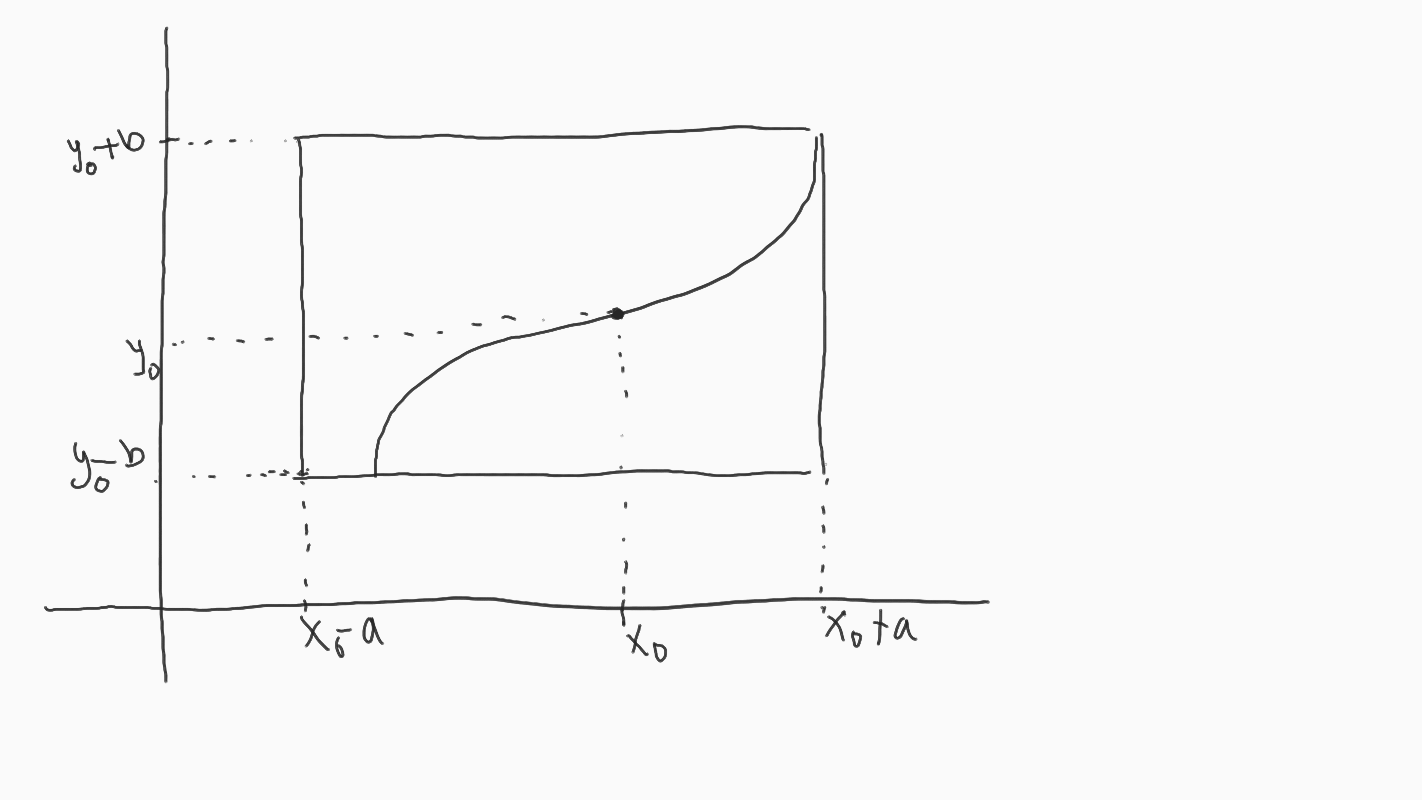
\includegraphics[scale=0.25]{graficas1.png}
    \caption{Caption}
    \label{fig:my_label}
\end{figure}


La condición de Lipschitz 
$$
|f(x_1,y_1)-f(x_2,y_2)|\leq N(y_1-y_2)
$$
puede ser sustituida por otra más fuerte, pero más fácilmente comprobable, la existencia de $\partial_{y} f^{'}$ en $D$ y que sea acotada.

En efecto para $(x,y)\in D$ y $|f'_y(x,y)|\leq N$ entonces por el teorema del valor intermedio:
$$
|f(x_1,y_1)-f(x_2,y_2)|=|f'_y(x,\xi)|-|y_1-y_2| 
$$
con $\xi\in (y_1,y_2)$. Así $(x,\xi)\in D$ y $|f_y(x,\xi)|\leq N$ , $|f(x,y_1)-f(x,y_2)|\leq N|y_1-y_2|$.

\begin{proof}
Observemos primero que 
$$
\left.\begin{array}{cc}
    \dfrac{\mathrm{d}y}{\mathrm{d}x}&=f(x,y)  \\
    &\\
    y(x_0) &=y_0 
\end{array}\right.
$$
es equivalente a
$$
y=y_0+\int_{x_0}^xf(x,y)\mathrm{d}x
$$

En efecto:
$$
\int_{x_0}^x\frac{\mathrm{d}y}{\mathrm{d}x}\mathrm{d}x=\int_{x_0}^xf(x,y)\mathrm{d}x
$$
así
$$
y(x)-y(x_0)=\int_{x_0}^xf(x,y)\mathrm{d}x
$$
y por tanto
$$
y(x)=y_0+\int_{x_0}^xf(x,y)\mathrm{d}x
$$
Ahora, hagamos una aproximación de  la solución 
\end{proof}

%----------------------------------------------------------------------------------------
%	Capitulo 3
%----------------------------------------------------------------------------------------
\chapter{Sistemas Lineales Planos y Ecuaciones de Orden Superior}


%----------------------------------------------------------------------------------------
%	Capitulo 4
%----------------------------------------------------------------------------------------
\chapter{Sistemas Tres Dimensionales y Sistemas No Lineales}

%----------------------------------------------------------------------------------------
%	Capitulo 5
%----------------------------------------------------------------------------------------
\chapter{Atractores Extraños y Caos}

%----------------------------------------------------------------------------------------
%	Capitulo 6
%----------------------------------------------------------------------------------------
\chapter{Teoría de Estabilidad}

%----------------------------------------------------------------------------------------
%	Capitulo 6
%----------------------------------------------------------------------------------------
\chapter{Sistemas Conservativos y Disipativos}



%----------------------------------------------------------------------------------------
%	BIBLIOGRAPHY
%----------------------------------------------------------------------------------------

\chapter*{Bibliography}
\addcontentsline{toc}{chapter}{\textcolor{ocre}{Bibliography}}
\section*{Books}
\addcontentsline{toc}{section}{Books}
\printbibliography[heading=bibempty,type=book]
\section*{Articles}
\addcontentsline{toc}{section}{Articles}
\printbibliography[heading=bibempty,type=article]

%----------------------------------------------------------------------------------------
%	INDEX
%----------------------------------------------------------------------------------------

\cleardoublepage
\phantomsection
\setlength{\columnsep}{0.75cm}
\addcontentsline{toc}{chapter}{\textcolor{ocre}{Index}}
\printindex

%----------------------------------------------------------------------------------------

\end{document}
